\documentclass{standalone}
\usepackage{tikz}
\usepackage{siunitx} % Para la notación de unidades

\begin{document}

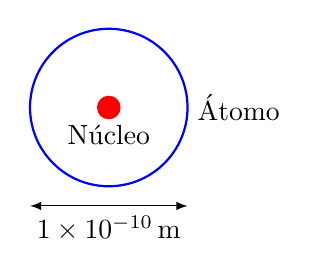
\begin{tikzpicture}
    % Núcleo
    \fill[red] (0,0) circle (0.15cm) node[black,yshift=-0.35cm] {Núcleo};
    % Órbita circular del electrón
    \draw[blue,thick] (0,0) circle (1cm) node[black,xshift=1.65cm] {Átomo};

    % Escala
    \draw[latex-latex] (-1,-1.25)--(1,-1.25);
    \node[below] at (0,-1.25){\SI{1e-10}{m}};
\end{tikzpicture}

\end{document}
